\chapter{Additional notes}

\section{The control vector separation for alignment is the Gouy phase separation}
% also the fact that mode matching is a constraint
\label{sec:gouysep}
A servo system which is designed to control several degrees of freedom of a system simultaneously must be able to effectively sense and control each degree of freedom independently. %NL%
The degrees of freedom of the system define a phase space, and the sensors and actuators can be represented as vectors in this space. %NL%
Where the components of the vectors have amplitudes proportional to the sensitivity of the sensor, or the actuation strength of the actuator, in a given degree of freedom. %NL%
In order to effectively control one's system, care should be taken to ensure that these vectors sufficiently span the phase space. %NL%
If any direction does not have coverage, it will either be unsensed, or uncontrolled.

In the case of the alignment of a laser beam, there are four degrees of freedom. %NL%
These may be parametrized as the beam waist position and beam waist angle in the $x$ and $y$ directions.\footnote{Where $z$ is the direction of propagation.} For good alignment control of a laser beam using steering mirrors, for example into an optical cavity, a common piece of lore is that one must have a steering mirror `close' to the alignment target, and one steering mirror `far' from it. %NL%
But just what exactly sets the criteria for close and far?

Let us constrain ourselves to a single plane of beam alignment, such that we are only concerned with the waist position and angle in the $x$ direction. %NL%
It can be shown that the field of the beam can be represented as the \TEM{00} field with some small additional \TEM{01} field added when the displacements and misalignments are small \cite{Anderson1984}. %NL%
To first order in misalignment, the field can be written as
\begin{equation}
\label{eqn:shifttilt}
\vect{E}=\vect{00}+\left(\frac{\delta x}{w_0} + i \frac{\theta}{\theta_d}\right)\vect{01}
\end{equation}
where $\vect{mn}$ is the \TEM{mn} eigenmode, $\delta x$ is the beam position displacement, $w_0$ is the beam waist radius, $\theta$ is the beam tilt angle, and $\theta_d=\lambda/(\pi w_0)$ is the divergence angle. %NL%
Therefore we may frame the problem of controlling the beam position and angle by our ability to control the real and imaginary quadratures of the amplitude of the \TEM{01} component. %NL%
Thus a `good' alignment system will be one in which the ability of the system to actuate on the real and imaginary quadratures of the \TEM{01} field is well separated.

We will represent our alignment system as two steering mirrors labeled A and B. %NL%
The beam first reflects from mirror A, travels some distance, then reflects from mirror B. %NL%
We will consider a vector space of the \TEM{00} and \TEM{01} modes as basis vectors. %NL%
From Equation \ref{eqn:mirrortilt} we see that, in this representation, the operator for mirror A is
\begin{equation}
%\oper{M}_{\rm A}=\oper{I}-2i\Theta_{\rm A}\left(\vect{00}\form{01}+\vect{01}\form{00}\right),
\oper{M}_{\rm A} \doteq \ms 1 &-2i\Theta_{\rm A}\\-2i\Theta_{\rm A} & 1\me
\end{equation}
where $\Theta_{\rm A}$ is the alignment angle of mirror A. %NL%
A similar expression holds for mirror B.

Between mirrors A and B, we allow the laser to propagate some distance. %NL%
Along with the propagation phase which is common to all modes, the \TEM{01} mode experiences the additional Gouy phase $\eta$. %NL%
The propagation operator is
\begin{equation}
%\oper{P}=e^{i\phi}\left(\vect{00}\form{00}+e^{i\eta}\vect{01}\form{01}\right),
\oper{P}\doteq e^{i\phi}\ms 1&0\\0&e^{i\eta}\me
\end{equation}
where $\phi$ is the overall phase common to all modes.

To first order in angles and ignoring the overall phase, the operator of the entire alignment system is
\begin{equation}
\oper{M}_{\rm B}\oper{P}\oper{M}_{\rm A}\doteq
\ms 1 & -2i\left(\Theta_{\rm A}+e^{i\eta}\Theta_{\rm B}\right)\\
-2i\left(e^{i\eta}\Theta_{\rm A}+\Theta_{\rm B}\right) & e^{i\eta} \me.
\end{equation}
If we apply this to a pure \TEM{00} field on the input, the output field is
\begin{equation}
\vect{E}_{\rm{out}}=\vect{00}-2i\left(e^{i\eta}\Theta_{\rm A}+\Theta_{\rm B}\right)\vect{01}.
\end{equation}
Comparing this to Equation \ref{eqn:shifttilt}, we see that mirror B actuates exclusively on the beam angle, while for mirror A, the amount of position or angle actuation depends on the Gouy phase propagation between the two mirrors, $\eta$. %NL%
If $\eta=\pi/2$, then mirror A only actuates on position and the two actuators are completely separated in actuator phase space. %NL%
In fact, the angle between the actuators in phase space is just $\eta$.

Intuitively, this may be understood by the fact that the \TEM{01} mode has an extra rotation relative to the \TEM{00} mode, this is the Gouy phase. %NL%
Once one of the mirrors has actuated on the beam, we must let the quadrature that was actuated on rotate away so that we may actuate on the perpendicular quadrature. %NL%
This rotation is what causes angles in the near field to rotate into positions in the far field. %NL%


The treatment of sensing is quite similar, in that case, it is the demodulation operator (Equation \ref{eqn:spacedemod}) which connects the \TEM{00} and \TEM{01} modes, and again, the Gouy phase dictates the sensor separation.

As a final thought, if one were designing an actuation system for modes of higher order than \TEM{01}, the propagation operator matrix element for a \TEM{mn} mode would be $e^{(m+n)\eta}$. %NL%
This would cause the optimal control separation (a phase space angle of $\pi/2$) to occur at $\eta=\frac{1}{m+n}\frac{\pi}{2}$. %NL%
Thus, mode matching sensors and actuators, which operate on $m+n=2$ modes, must have  $\eta=\pi/4$ separation for optimal performance.

\section{Dither sensing is a measurement of a partial derivative}
\label{sec:dithersens}
Suppose one has a sensor which measures some physical quantity $P$, which depends on a variable $\theta$ which is controlable by some means of actuation. %NL%
A modulation is injected into the variable $\theta$ such that
\begin{equation}
\theta = \theta_0+\alpha \sin[\omega t],
\end{equation}
where $\alpha \ll 1$ is the modulation depth, and $\omega$ is the modulation frequency. %NL%
The resulting behavior of $P$ is
\begin{equation}
P(\theta)=P(\theta_0+\alpha \sin[\omega t])\approx P(\theta_0)+\frac{\partial P}{\partial \theta}(\theta_0)\alpha \sin[\omega t] + \ldots
\end{equation}
Thus the amplitude of the $\omega$ frequency component, which can be determined by demodulation, is proportional to the partial derivative of the measured quantity with respect to the controlled variable. %NL%
This is the basic mechanism behind dither sensing.
\section{Conventions for the coefficient of amplitude transmission and reflectivity of beamsplitters}
Imagine a beam with complex electric field amplitude $E_0$ striking a partially reflective boundary. %NL%
The beam will be split into two resultant beams, a transmitted beam and reflected. %NL%
Define the transmitted beam as a complex coefficient, $t$, multiplied by the incident beam. %NL%
Similarly, the reflected beam will be multiplied by $r$. %NL%
This is shown in Figure \ref{fig:mrfig1}. %NL%
Note: we make no assumption about the value of these coefficients. %NL%
At all times we will ignore phase shifts due simply to propagation, so the $ik\delta z$ phase is always divided out.

\begin{figure}
  \begin{center}
  \leavevmode
  \subfloat[The incident beam.]{\label{fig:mrfig1}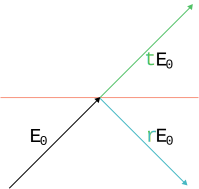
\includegraphics{figs-ap-notes/mrfig1.pdf}}
  ~
  \subfloat[The time reversed situation.]{\label{fig:mrfig2}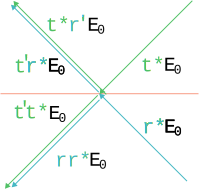
\includegraphics{figs-ap-notes/mrfig2.pdf}}
  \end{center}
  \caption{Diagram of the interaction of a beam with a beamsplitter.}
  \label{fig:mrfig}
\end{figure}

Imagine the time reversed process of the two resultant beams. %NL%
In the phasor space of the electric field, time reversal requires the complex conjugation operation. %NL%
The blue beam will be split into two beams for which we will use the same coefficients of transmission and reflection as in the case already considered, because it interacts with the boundary from the same direction. %NL%
However, we will assume that the green beam, which is hitting the boundary from the other side, has different coefficients, $t'$ and $r'$. %NL%
This situation is shown in Figure \ref{fig:mrfig2}.

Now, we make the assumption that this process obeys the principal of time reversal symmetry.\footnote{This also implicitly assumes there are no losses.} Thus the result of the second case should match the initial conditions of the first case. %NL%
The the two beams above the boundary should interfere destructively, while the two below should reproduce the original input beam. %NL%
This gives us two equations.
\begin{align*}
rr^*+t't^*&=1,\\
t'r^*+r't^*&=0.
\end{align*}
Solving for $t$ gives
\begin{equation}
t=-ie^{i\phi/2}\sqrt{1-|r|^2},
\end{equation}
where $e^{i\phi}\equiv r'/r^*$. %NL%
The two most common conventions choose $r$ to be real and $\phi$ to either be $\pi$, leading to the $r=-r'$ with $t$ real convention, or $2\pi$, leading to the $r=r'$ with $t=i\tau$ for $\tau$ real convention.

\section{The focusing power of a displaced mirror}
When optimizing the mode matching of a laser beam into an optical cavity, there are typically two ways to modify the focusing of the beam. %NL%
One is to change the optical elements for others with a differing focal length, or in some extreme cases, by using optical elements with a variable focusing power (Chapter \ref{ch:modematching}). %NL%
The second method is to modify the position of the optical elements, this changes the free propagation distance between the elements, and hence, the locations and sizes of the focused beams.

The question to be addressed is ``How does one compare a change in focal length to a change in position of the optic in a quantitatively equivalent way?'' %NL%
For small perturbations of mode matching, a change in the focus of a beam can be considered as coupling between the \TEM{00} mode with the second order ($m+n=2$) modes of the beam \cite{Anderson1984}. %NL%
For a variable focusing power, this is given in Equation \ref{eq:matrixelement}. %NL%
Here we aim to calculate a similar expression for a mirror \com{and a lens?} that has been displaced along the optic axis.

\com{TBD}
\section{The second order HOMs}

\begin{figure}[h!]
  \begin{center}
  \leavevmode
  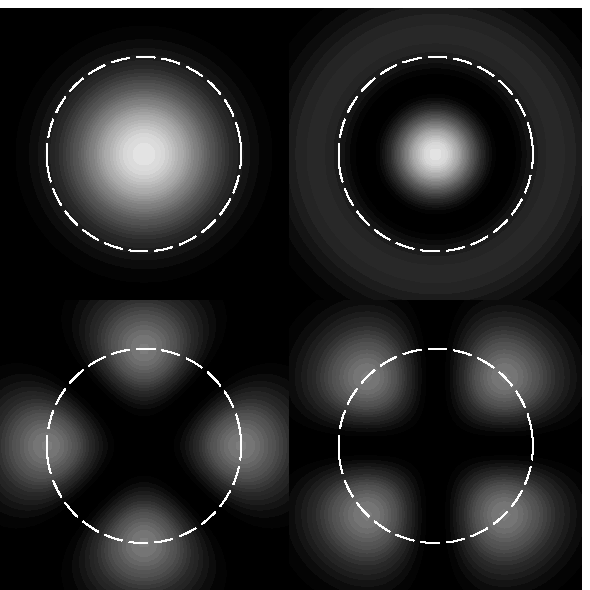
\includegraphics{figs-ap-notes/puresecondordermodes.pdf}
  \end{center}
  \caption[Visualization of the second order modes.]{Visualization of the second order modes. The top left panel shows a pure \TEM{00} mode. The bull's-eye mode is shown in the top right panel. The lower left panel shows the astigmatic mode along the horizontal and vertical axes. The lower right panel shows the astigmatic mode along the 45\degrees{} axes. For reference, a dashed circle is drawn to outline the beam width radius of the \TEM{00} mode.}
  \label{fig:puresecondordermodes}
\end{figure}

\begin{figure}[h!]
  \begin{center}
  \leavevmode
  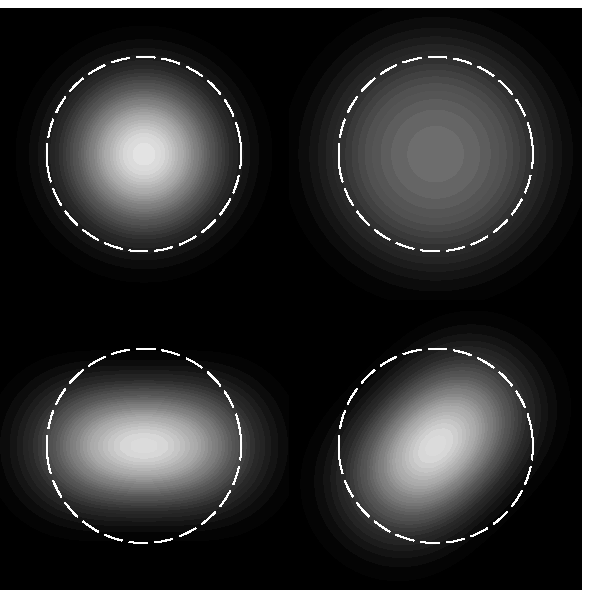
\includegraphics{figs-ap-notes/secondordermodes.pdf}
  \end{center}
  \caption[The effects of second order mode perturbations on the \TEM{00} mode.]{The effects of second order mode perturbations on the \TEM{00} mode. A pure \TEM{00} mode is shown  in the top left panel. The top right panel shows how the bull's-eye mode alters the beam radius. The two bottom panels show how the astigmatic modes modify the pure beam. For reference, a dashed circle is drawn on all panels at the beam width radius of the pure \TEM{00} mode.}
  \label{fig:secondordermodes}
\end{figure}
Various higher order modes are often visualized in terms of the intensity profile of a given pure mode. %NL%
This can be useful in conveying how the intensity of different modes are distributed. %NL%
Another useful way to visualize the modes is to consider the perturbation of the \TEM{00} mode when a new mode is added. %NL%
In the case of alignment, this is useful in showing that the addition of some amount of \TEM{01} mode acts to displace the beam horizontally.

Figure \ref{fig:puresecondordermodes} shows the \TEM{00} mode along with the three second order modes. %NL%
The \TEM{00} mode is shown in the top left panel. %NL%
The top right panel shows the bull's-eye mode, or $(U_{20}+U_{02})/\sqrt{2}$. %NL%
The lower left panel shows $(U_{20}-U_{02})/\sqrt{2}$, and the lower right panel shows the \TEM{11} mode, $U_{11}$.

Just as the first order modes are responsible for beam misalignments, the second order modes are responsible for mode mismatching. %NL%
This can be seen by visualizing the change in the intensity profile of a beam when some small amount of second order mode perturbation is added. %NL%
Figure \ref{fig:secondordermodes} shows the effects of the second order modes on a \TEM{00} beam. %NL%
The top left panel is a pure \TEM{00} beam, for reference. %NL%
The top right shows the effect of adding about 20\perc{} of the bull's-eye mode in amplitude. %NL%
The center peak has been suppressed and field has been added to the outer edges of the beam. %NL%
This causes the beam to spread out and have a larger beam size. %NL%
The lower panels show the effects of the two astigmatic modes. %NL%
The $(U_{20}-U_{02})/\sqrt{2}$ mode is responsible for astigmatism along the vertical and horizontal axes, while the \TEM{11} mode is responsible for astigmatism along the axes rotated by 45\degrees{}.
